
\chapter{Foundations of Topology}
Now we can generalize our observations on metric spaces to topological spaces:
\begin{definition}[Topological Space] A topological space $(X, \mathcal{T})$ consists of a (non-empty) set \(X\), and a family of subsets $\mathcal{T}$ of \(X\) such that:

1. \(\varnothing,X \in  \mathcal{T}\)

2. \(U,V \in  \mathcal{T}\) implies \(U \cap  V \in  \mathcal{T}\)

3. If \({U}_{\alpha} \in  \mathcal{T}\) for all \(\alpha  \in  \mathcal{A}\), then \(\mathop{\bigcup}\limits_{{\alpha  \in  \mathcal{A}}}{U}_{\alpha} \in  \mathcal{T}\).

The elements in \(\mathcal{T}\) are called \emph{open subsets} of \(X\). The \(\mathcal{T}\) is called a topology on \(X\).
\end{definition}

Obviously, for any metric space $(X,d)$, the set
\[
\mathcal{T} = \{ \text{all open subsets of}X\}
\]
defines a topology on \(X\).

\begin{definition} 
For any set $X$, define the discrete topology by
\[
\mathcal{T}_{\mathrm{dis}} := \{ \text{all subsets of }X\}
\]
It’s clear that \(\mathcal{T}_{\mathrm{dis}}\) is a topology on \(X\)
\end{definition}
Note that if we use the discrete metric \(\left({X,d_{\mathrm{dis}}}\right)\), then all subsets are open sets. So we say 
$(X, \mathcal{T}_{\mathrm{dis}})$ is {\bf induced} from the discrete metric $(X, d_{\mathrm{dis}})$. More generally, we say $(X,\mathcal{T})$ is metrizable if \(\mathcal{T}\) is precisely the family of open subsets of some metric $d$ of $X$.

Here is another extreme of topology with the smallest possible number of open sets:
\begin{example}
Let \(X\) be a set containing more than one element. Consider the indiscrete topology \(\left({X,{\mathcal{T}}_{\text{indis}}}\right)\), where:
\[
{\mathcal{T}}_{\text{indis}} = \{ \varnothing,X\} \text{.}
\]
Once again, it is easy to check that it defines a topology of $X$. 

Now we explore whether \(\left({X,{\mathcal{T}}_{\text{indis}}}\right)\) is metrizable or not. Firstly, note that for any metric \(d\) defined on \(X\), let \(x,y\) be distinct points in \(X\). Then \(\varepsilon  := d\left({x,y}\right)  > 0\), hence \({B}_{\frac{1}{2}\varepsilon}\left(x\right)\) is a open set belonging to the corresponding induced topology. Since \(x \in  {B}_{\frac{1}{2}\varepsilon}\left(x\right)\) and \(y \notin  {B}_{\frac{1}{2}\varepsilon}\left(y\right)\), we conclude that \({B}_{\frac{1}{2}\varepsilon}\left(x\right)\) is neither \(\varnothing\) nor \(X\), i.e., the topology induced by any metric \(d\) is not the indiscrete topology.
\end{example}

\begin{example}
For any set $X$, consider the cofinite topology \(\left({X,{\mathcal{T}}_{\text{cofin}}}\right)\) :

\[
{\mathcal{T}}_{\text{cofin}} = \{ U \mid  X \smallsetminus  U\text{is a finite set}\} \bigcup \{ \varnothing \}
\]
(Question - is \(\left({X,{\mathcal{T}}_{\text{cofin}}}\right)\) metrizable?)
\end{example}

\begin{definition} [Equivalence] Two metrics $d_1, d_2$ of $X$ are topologically equivalent if they give rise to the same topology.
\end{definition}

For instance, the metrics \({d}_{1},{d}_{2},{d}_{\infty}\) in \({\mathbb{R}}^{n}\) are topologically equivalent.

\begin{definition}[Closed set] Let $(X, \mathcal{T})$ be a topological space. Then \(V \subseteq  X\) is closed if \(X \smallsetminus  V \in  \mathcal{T}\)
\end{definition}
\begin{example} Under the usual topology \(\left({\mathbb{R},{\mathcal{T}}_{\text{usual}}}\right)\), \(\left({b,\infty}\right)  \cup  \left({-\infty,a}\right)  \in  \mathcal{T}\). Therefore,
\[
\left\lbrack  {a,b}\right\rbrack   = \mathbb{R} \smallsetminus  \left({\left({b,\infty}\right) \bigcup \left({-\infty,a}\right)}\right)
\]
is closed in \(\mathbb{R}\) under usual topology.
\end{example}

It is {\bf important} to say that \(V\) is closed in \(X\). You need to specify the underlying the space \(X\).

\begin{proposition} Let $(X, \mathcal{T})$ be a topological space. 

1. \(\varnothing,X\) are closed in \(X\)

2. \({V}_{1},{V}_{2}\) closed in \(X\) implies that \({V}_{1} \cup  {V}_{2}\) closed in \(X\)

3. \(\left\{  {{V}_{\alpha} \mid  \alpha  \in  \mathcal{A}}\right\}\) closed in \(X\) implies that \(\mathop{\cap}\limits_{{\alpha  \in  \mathcal{A}}}{V}_{\alpha}\) closed in \(X\)
\end{proposition}

\begin{proof} (1) is obvious. For (2) and (3), one can apply De Morgan's Law
\(\left({X \smallsetminus  \mathop{\bigcup}\limits_{{i \in  I}}{U}_{i}}\right)  = \mathop{\cap}\limits_{{i \in  I}}\left({X \smallsetminus  {U}_{i}}\right)\)
\end{proof}

\section{Convergence}
Inspired by the discussions in Chapter 1 on metric spaces, we have:
\begin{definition}[Convergence] A sequence \(\left\{  x_n\right\}\) of a topological space $(X, \mathcal{T})$ converges to \(x \in  X\) if for all open \(\ U \ni  x\), there exists \(N\) such that \(x_n \in  U,\forall n \geq  N\).
\end{definition}

\begin{example} \begin{enumerate}
    \item For the usual topology \(\left({X = {\mathbb{R}}^{n},{d}_{2}}\right)  \rightarrow  \left({X,\mathcal{T}}\right)\), convergence of sequence in \(\left({{\mathbb{R}}^{n},\mathcal{T}}\right)\) is the usual convergence in analysis.
    
    Note that for \({\mathbb{R}}^{n}\) or metric space, the limit of sequence (if exists) is unique. However, this is no longer true if the topology is not metrizable.

\item Consider the topological space \(\left({X,{\mathcal{T}}_{\text{indis}}}\right)\). Take any sequence \(\left\{  x_n\right\}\) in \(X\), it is convergent to any \(x \in  X\). Indeed, For all \(U \ni  x\) open, the only possibility is \(U = X\). Therefore,
\[
x_n \in  U\left({ = X}\right),\forall n \geq  1\text{.}
\]

\item Consider the topological space \(\left({X,{\mathcal{T}}_{\text{cofin}}}\right)\), where \(X\) is infinite. Consider \(\left\{  x_n\right\}\) is a sequence satisfying \(m \neq  n\) implies \(X_{m} \neq  x_n\). Then \(\left\{  x_n\right\}\) is convergent to any \(x \in  X\). 

\item Consider the topological space \(\left({X,{\mathcal{T}}_{\text{discrete}}}\right)\), the sequence \(\left\{  x_n\right\}   \rightarrow  x\) is equivalent to saying \(x_n = x\) for all sufficiently large \(n\).
\end{enumerate}
\end{example}

One lesson we learned from the previous example is that the limit of sequences may not be unique. In such a case, the reason is that \(\mathcal{T}\) is not "big enough". We will give a criterion to make sure the limit is unique in the future. (Hausdorff)

\begin{proposition} If \(F \subseteq  \left({X,\mathcal{T}}\right)\) is closed, then for any convergent sequence \(\left\{  x_n\right\}\) in \(F\), the limit(s) are also in \(F\).
\end{proposition}
\begin{proof} Let \(\left\{  x_n\right\}\) be a sequence in \(F\) with limit \(x \in  X\). Suppose on the contrary that \(x \notin  F\) (i.e., \(x \in  X \smallsetminus  F\) that is open). There exists \(N\) such that
\[
x_n \in  X \smallsetminus  F,\forall n \geq  N
\]
i.e., \(x_n \notin  F\), which is a contradiction.
\end{proof}

If the $(X, \mathcal{T})$ is metrizable, the converse holds. Otherwise, the converse may not be true. 
\begin{example} Consider the co-countable topological space \(\left({X = \mathbb{R},{\mathcal{T}}_{\text{co-count}}}\right)\), where
\[
{\mathcal{T}}_{\mathrm{{co-count}}} = \{ U \mid  X \smallsetminus  U\text{is a countable set}\} \bigcup \{ \varnothing \},
\]
and \(X\) is uncountable. Then note that \(F = \left\lbrack  {0,1}\right\rbrack   \subsetneqq  X\) is an un-countable set, and under co-countable topology, \(F \supseteq  \left\{  x_n\right\}   \rightarrow  x\) implies \(x_n = x \in  F\) for all \(n\). It is clear that \(X \smallsetminus  F \notin  {\mathcal{T}}_{\mathrm{{co-count}}}\), that is, \(F\) is not closed.
\end{example}

\section{Interior, Closure, Boundary}
\begin{definition} \label{def:interior_closure} Let $(X, \mathcal{T})$ be a topological space, and \(A \subseteq  X\) a subset.

1. The interior of \(A\) is

\[
{A}^{ \circ } = \mathop{\bigcup}\limits_{{U \subseteq  A,U\text{ is open}}}U
\]

2. The closure of \(A\) is
\[
\bar{A} = \mathop{\bigcap}\limits_{{A \subseteq  V,V\text{ is closed}}}V
\]
If \(\bar{A} = X\), we say that \(A\) is dense in \(X\).
\end{definition}

The above definition can be illustrated as follows:
\begin{center}
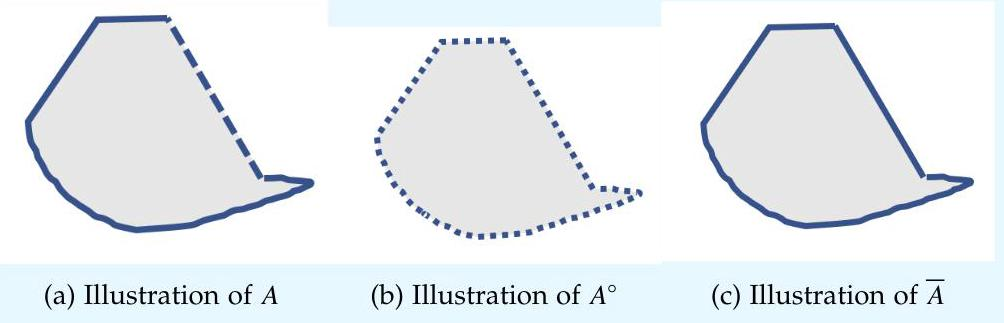
\includegraphics[width=0.6\textwidth]{images/Ch2_interior_closure.jpg}
\end{center}

\begin{example}
\begin{itemize}
\item For \(\lbrack a,b) \subseteq  \mathbb{R}\), we have:
\[
\lbrack a,b{)}^{ \circ } = \left({a,b}\right),\;\overline{\lbrack a,b)} = \left\lbrack  {a,b}\right\rbrack
\]

\item For \(X = \mathbb{R},{\mathbb{Q}}^{ \circ } = \varnothing\) and \(\overline{\mathbb{Q}} = \mathbb{R}\).

\item Consider the discrete topology \(\left({X,{\mathcal{T}}_{\text{discrete}}}\right)\), we have
\[
{S}^{ \circ } = S,\;\bar{S} = S
\]
\end{itemize}
\end{example}

The insights behind \autoref{def:interior_closure} is as follows:
\begin{proposition}
\leavevmode \medskip
\begin{enumerate}
    \item  \({A}^{ \circ }\) is the largest open subset of \(X\) contained in \(A\) ;

\item \(\bar{A}\) is the smallest closed subset of \(X\) containing \(A\).

\item If \(A \subseteq  B\), then \({A}^{ \circ } \subseteq  B\) and \(\bar{A} \subseteq  \bar{B}\)

\item \(A\) is open in \(X\) is equivalent to say \({A}^{ \circ } = A;A\) is closed in \(X\) is equivalent to say \(\bar{A} = A\).
\end{enumerate}
\end{proposition}

\begin{example} Let $(X, d)$ be a metric space. What’s the closure of an open ball \({B}_{r}\left(x\right)\) ? The direct intuition is to define the closed ball
\[
{\bar{B}}_{r}\left(x\right)  = \{ y \in  X \mid  d\left({x,y}\right)  \leq  r\}.
\]
One would like to know whether \({\bar{B}}_{r}\left(x\right)  = \overline{{B}_{r}\left(x\right)}\). Indeed, since \({\bar{B}}_{r}\left(x\right)\) is a closed subset of \(X\), and \({B}_{r}\left(x\right)  \subseteq  {\bar{B}}_{r}\left(x\right)\), we imply that
\[
\overline{{B}_{r}\left(x\right)} \subseteq  {\bar{B}}_{r}\left(x\right)
\]
However, we may find an example such that \(\overline{{B}_{r}\left(x\right)}\subsetneq {\bar{B}}_{r}\left(x\right)\) - consider the discrete metric space \(\left({X, d_{\mathrm{dis}}}\right)\). Then for all \(x \in  X\),
\[
B_1\left(x\right)  = \{ x\}  \Rightarrow  \overline{B_1\left(x\right)} = \{ x\},\;{\bar{B}}_{1}\left(x\right)  = X
\]
The equality \({\bar{B}}_{r}\left(x\right)  = \overline{{B}_{r}\left(x\right)}\) holds when $(X, d)$ is a normed space.
\end{example}

Here is another characterization of \(\bar{A}\): 
\begin{proposition} \label{prop:closure_of_A}
\[
\bar{A} = \{ x \in  X \mid \mathrm{for\ all\ open\ }U \ni  x,\ U\cap A \neq  \varnothing \}
\]
\end{proposition}

\begin{proof} Define
\[
S = \{ x \in  X \mid  \text{for all open }U \ni  x,U \cap  A \neq  \varnothing \}
\]
It suffices to show that \(\bar{A} = S\): 

\noindent{Claim:} \(S\) is closed, or equivalently $X \smallsetminus  S$ is open: Note that
\[
X \smallsetminus  S = \left\{  {x \in  X\mid \exists\ U_x \ni  x\text{ open such that }U_x \cap  A = \varnothing}\right\}
\]
Take \(x \in  X \smallsetminus  S\), i.e. there exists open \(U_x \ni  x\) such that \(U_x \cap  A = \varnothing\). Then our claim follows if one can prove that
\[U_x \subseteq  X \smallsetminus  S.\]
Indeed, for all \(y \in  U_x\), since \(U_x \ni  y\) and \(U_x \cap  A = \varnothing\) by definition, hence 
\(y \in  X \smallsetminus  S\).
Therefore, 
\[
X \smallsetminus  S = \mathop{\bigcup}\limits_{{x \in  X \smallsetminus  S}}\{ x\}  \subseteq  \mathop{\bigcup}\limits_{{x \in  X \smallsetminus  S}}U_x \subseteq  X \smallsetminus  S,
\]
which implies \(X \smallsetminus  S = \mathop{\bigcup}\limits_{{x \in  X \smallsetminus  S}}U_x\) is open, i.e., \(S\) is closed in \(X\) and the claim is proved.

Now go back to the proof. By definition, it is clear that \(A \subseteq  S\), since
\[
\forall a \in  A,\forall \text{ open }U \ni  a,\ U\cap A \supseteq  \{ a\}  \neq  \varnothing
\]
which implies that $a \in  S$. Therefore, 
\[\bar{A} \subseteq  \bar{S} = S\]
by the above claim. And one needs to show it is an equality.

Suppose on contrary that there exists \(y \in  S \smallsetminus  \bar{A}\). Since \(y \notin  \bar{A}\), by definition, there exists \(F \supseteq  A\) closed such that \(y \notin  F\).
Therefore, \(y \in  X \smallsetminus  F\) that is open, and
\[
\left({X \smallsetminus  F}\right) \cap A \subseteq  \left({X \smallsetminus  A}\right) \cap A = \varnothing  \Rightarrow  y \notin  S,
\]
which is a contradiction. Therefore, \(S = \bar{A}\).
\end{proof}

\begin{definition}[Accumulation point] Let \(A \subseteq  X\) be a subset in a topological space. We call \(x \in  X\) an \emph{accumulation point (limit point)} of \(A\) if
\[
\mathrm{for\ all\ } U \subseteq  X \mathrm{\ open\ such\ that\ }U \ni  x,\left({U\smallsetminus \{ x\}}\right) \cap A \neq  \varnothing.
\]
\end{definition}

\begin{example}
\begin{enumerate}
    \item There exists some point in \(A\) but not in \({A}^{\prime}\) :
\[
A = \{ 1,2,3,\ldots,n,\ldots \}
\]
Then any point in \(A\) is not in \({A}^{\prime}\).

\item There also exists some point in \({A}^{\prime}\) but not in \(A\) :
\[
A = \left\{  {\left. \frac{1}{n}\right| \;n \geq  1}\right\}
\]
Then the point 0 is in \({A}^{\prime}\) but not in \(A\).
\end{enumerate} 
\end{example}

\begin{proposition} \(\bar{A} = A\bigcup {A}^{\prime}\).
\end{proposition}

\begin{proof} This proposition directly follows from \autoref{prop:closure_of_A} and the definition of \({\mathrm{A}}^{\prime}\).
\end{proof}

\begin{definition}[Sequential Closure] Let \({A}_{S}\) be the set of limits of any convergent sequence in \(A\), then \({A}_{S}\) is called the sequential closure of \(A\).
\end{definition}

\begin{lemma}Retain the above notations. Then 
\[A \subseteq  {A}_{S} \subseteq  \bar{A}.\]
\end{lemma}
\begin{proof}
It is clear that \(A \subseteq  {A}_{S}\), since the sequence \(\left\{  {{a}_{n} := a}\right\}\) for all $n \in \mathbb{N}$ is convergent to \(a\) for all \(a \in  A\).

For the other inclusion, suppose \(a \in  {A}_{S}\). Then we have \(\left\{  {a}_{n}\right\} \rightarrow  a\) for some sequence $\{a_n\}$. Therefore, for any open \(U \ni  a\), there exists \(N\) such that \(\left\{  {{a}_{N},{a}_{N + 1},\ldots}\right\}   \subseteq  U \cap  A \neq  \varnothing\). Therefore, \(a \in  \bar{A}\), i.e., \({A}_{S} \subseteq  \bar{A}\).
\end{proof}


We would like to know if the sequential closure is equal to the closure. And the answer is yes for metric spaces:
\begin{proposition} Let $(X, d)$ be a metric space, then \({A}_{S} = \bar{A}\).
\end{proposition}
\begin{proof} In view of the lemma above, one only needs to prove the inclusion $\bar{A} \subseteq A_S$. 

Let \(a \in  \bar{A}\), then there exists \({a}_{n} \in  {B}_{1/n}\left(a\right)  \cap  A\), which implies \(\left\{  {a}_{n}\right\}   \rightarrow  a\), i.e., \(a \in\)  \({A}_{S}\).
\end{proof}

Indeed, the same result goes for first countable topological spaces. However, \({A}_{S}\) is a proper subset of \(\bar{A}\) in general: Let \(A \subseteq  X\) be the set of continuous functions, where \(X = {\mathbb{R}}^{\mathbb{R}}\) denotes the set of all real-valued functions on \(\mathbb{R}\), with the topology of pointwise convergence. Then \({A}_{S} = B_1\), the set of all functions of first Baire-Category on \(\mathbb{R}\) ; and \({\left\lbrack  {A}_{S}\right\rbrack }_{S} = B_2\), the set of all functions of second Baire-Category on \(\mathbb{R}\). Since \(B_1 \neq  B_2\), we have \({\left\lbrack  {A}_{S}\right\rbrack }_{S} = {A}_{S}\). Note that \(\overline{\bar{A}} = \bar{A}\). We conclude that \({A}_{S}\) cannot equal to \(\bar{A}\), since the sequential closure operator cannot be idempotent.

\begin{definition}[Boundary] The boundary of \(A\) is defined as

\[
\partial A = \bar{A} \smallsetminus  {A}^{\circ}
\]
\end{definition}

\begin{proposition} Let $(X, \mathcal{T})$ be a topological space with \(A,B \subseteq  X\). Then
\begin{enumerate}
    \item $\overline{X \smallsetminus  A} = X \smallsetminus  {A}^{ \circ },$
    \item $\quad{\left(X \smallsetminus  B\right)}^{ \circ } = X \smallsetminus  \bar{B}$,
    \item $\partial A = \bar{A} \cap  \left(\overline{X \smallsetminus  A}\right)$.
\end{enumerate}
\end{proposition}
\begin{proof}
\begin{enumerate}
    \item \(
X \smallsetminus  {A}^{ \circ } = X \smallsetminus  \left({\mathop{\bigcup}\limits_{{U\text{is open,}U \subseteq  A}}U}\right)  
= \mathop{\cap}\limits_{{U\text{is open,}U \subseteq  A}}\left({X \smallsetminus  U}\right)  
= \mathop{\cap}\limits_{{V\text{is closed,}F \supseteq  X \smallsetminus  A}}F 
= \overline{X \smallsetminus  A}\).
\item Denote \(B := X \smallsetminus  A\) by \(B\), we obtain:
\[
{\left(X \smallsetminus  B\right)}^{ \circ } = {A}^{ \circ } 
= X \smallsetminus  \left({X \smallsetminus  {A}^{ \circ }}\right)
= X \smallsetminus  \overline{X \smallsetminus  A} 
= X \smallsetminus  \bar{B}.
\]
\item By definition of \(\partial A\),
\[
\partial A = \bar{A} \smallsetminus  {A}^{ \circ } 
= \bar{A}\cap \left({X \smallsetminus  {A}^{ \circ }}\right)
= \bar{A}\cap \left(\overline{X \smallsetminus  A}\right) 
\]
\end{enumerate}
\end{proof}

\section{Functions on Topological Space}
We now study maps $f:X \to Y$ between topological spaces. As in linear algebra/abstract algebra, we would like our map to preserve certain properties of the spaces (e.g. we study {\bf linear transformations} for linear algebra, and {\bf group homomorphisms} for groups). 

In the case of topological spaces, we have:
\begin{definition}[Continuous Map] Let \(f : \left({X,{\mathcal{T}}_X}\right)  \rightarrow  \left({Y,{\mathcal{T}}_Y}\right)\) be a map. Then the function \(f\) is continuous, if
\[
U \in  {\mathcal{T}}_Y \Rightarrow  {f}^{-1}\left(U\right)  \in  {\mathcal{T}}_X
\]
\end{definition}

\begin{example}
1. The identity map id : \(\left({X,\mathcal{T}}\right)  \rightarrow  \left({X,\mathcal{T}}\right)\) defined as \(x \mapsto  x\) is continuous

2. The identity map id : \(\left({X,{\mathcal{T}}_{\text{discrete}}}\right)  \rightarrow  \left({X,{\mathcal{T}}_{\text{indiscrete}}}\right)\) defined as \(x \mapsto  x\) is continuous. Since \({\operatorname{id}}^{-1}\left(\varnothing \right)  = \varnothing\) and \({\operatorname{id}}^{-1}\left(X\right)  = X\)

3. The identity map id : \(\left({X,{\mathcal{T}}_{\text{indiscrete}}}\right)  \rightarrow  \left({X,{\mathcal{T}}_{\text{discrete}}}\right)\) defined as \(x \mapsto  x\) is not continuous.
\end{example}

\begin{proposition} \label{prop:comp_cont_is_cont} If \(f : X \rightarrow  Y\), and \(g : Y \rightarrow  Z\) be continuous, then \(g \circ  f\) is continuous
\end{proposition}

\begin{proof} For given \(U \in  {\mathcal{T}}_{Z}\), we imply
\[
{g}^{-1}\left(U\right)  \in  {\mathcal{T}}_Y \Rightarrow  {f}^{-1}\left({{g}^{-1}\left(U\right)}\right)  \in  {\mathcal{T}}_X,
\]
i.e., \({\left(g \circ  f\right)}^{-1}\left(U\right)  \in  {\mathcal{T}}_X\)
\end{proof}

The following proposition is well-known in calculus and metric spaces. This remains to be true for topological spaces:
\begin{proposition} Suppose \(f : X \rightarrow  Y\) is continuous between two topological spaces. Then \(\left\{  x_n\right\}   \rightarrow  x\) implies \(\left\{  {f\left(x_n\right)}\right\}   \rightarrow  f\left(x\right)\).
\end{proposition}

\begin{proof} Take open \(U \ni  f\left(x\right)\), which implies \({f}^{-1}\left(U\right)  \ni  x\). Since \({f}^{-1}\left(U\right)\) is open, we imply there exists \(N\) such that
\[
\left\{  {x_n \mid  n \geq  N}\right\}   \subseteq  {f}^{-1}\left(U\right)
\]
i.e., \(\left\{  {f\left(x_n\right)  \mid  n \geq  N}\right\}   \subseteq  U\)
\end{proof}

Here is the definition in topology analogous to isomorphism in algebra:
\begin{definition}[Homeomorphism] A homeomorphism between spaces topological spaces \(\left({X,{\mathcal{T}}_X}\right)\) and \(\left({Y,{\mathcal{T}}_Y}\right)\) is a bijection
\[
f : \left({X,{\mathcal{T}}_X}\right)  \rightarrow  \left({Y,{\mathcal{T}}_Y}\right)
\]
such that both \(f\) and \({f}^{-1}\) are continuous.
\end{definition}

{\bf WARNING:} In linear algebra and abstract algebra, if $f: X \to Y$ is a bijective linear transformation or homomorphism, then its inverse $f^{-1}: Y \to X$ is automatically a linear transformation or homomorphism. However, this is {\bf NOT TRUE} for topological spaces! Therefore, we need to decree that both $f$ and $f^{-1}$ are continuous in our definition above.

\begin{example}
    The sets $(0,\infty)$ and $\mathbb{R}$ are homeomorphic, since
    $$\mathrm{exp}: \mathbb{R} \to (0,\infty)$$
    is bijective and continuous, with inverse
    $$\log: (0,\infty) \to \mathbb{R}$$
    also being continuous.
\end{example}
\section{New Spaces From Old}

\subsection{Subspace Topology and Basis}
Let $A \subseteq X$ be a subset, we define a topology of $A$ from that of $X$:
\begin{definition} \label{def:subspace_topology} Let \(A \subseteq  X\) be a non-empty set. The subspace topology of \(A\) is defined by any of the equivalent ways:
\begin{enumerate}
\item \({\mathcal{T}}_{A} := \left\{  {U \cap  A \mid  U \in  {\mathcal{T}}_{X}}\right\}.\)
\item $\mathcal{T}_A$ is the coarsest topology on \(A\) such that the inclusion map
\[
i : \left({A,{\mathcal{T}}_{A}}\right)  \rightarrow  \left({X,{\mathcal{T}}_X}\right),\;i\left(x\right)  = x
\]
is continuous. (We say the topology \({\mathcal{T}}_{1}\) is coarser than \({\mathcal{T}}_{2}\), or \({\mathcal{T}}_{2}\) is finer than \({\mathcal{T}}_{1}\), if \({\mathcal{T}}_{1} \subseteq  {\mathcal{T}}_{2}\) e.g., \({\mathcal{T}}_{\text{discrete}}\) is the finest topology, and \({\mathcal{T}}_{\text{indiscrete}}\) is coarsest topology.)

\item $\mathcal{T}_A$ is the unique topology such that for any topological spaces \(\left({Y,{\mathcal{T}}_Y}\right)\),
\begin{center}
$f : \left({Y,{\mathcal{T}}_Y}\right)  \rightarrow  \left({A,{\mathcal{T}}_{A}}\right)$ is continuous iff \(i \circ  f : \left({Y,{\mathcal{T}}_Y}\right)  \rightarrow  \left({X,{\mathcal{T}}_X}\right)\) is continuous.
\end{center}
\end{enumerate}
\end{definition}

\begin{exercise} \label{ex:subspace_topology}
\leavevmode
\begin{enumerate}
    \item The definition (1) in \autoref{def:subspace_topology} does define a topology of \(A\).
\item The closed sets of \(A\) under subspace topology are of the form \(V \cap  A\), where \(V\) is closed in \(X\)
\item Show that (1) and (2) are equivalent (Hint: one can make sure of the easy fact that \(
{i}^{-1}\left(S\right)  = S\cap A
\) for all subsets $S$).
\end{enumerate}
\end{exercise}

\begin{example} Let all English and numerical letters be subset of \({\mathbb{R}}^{2}\). Then
\begin{center}
P, 6
\end{center}
are homeomorphic using the subspace topology.
\end{example}

\begin{proposition} \label{prop:subspace_equivalent} The statements in \autoref{def:subspace_topology} are equivalent.
\end{proposition}
\begin{proof} 
We only need to prove $(1) \Rightarrow (3)$ and $(3) \Rightarrow (1)$:


\(\mathbf{(1) \Rightarrow (3)}\): Suppose \(\mathcal{T}_A = \{U \cap A\ |\ U \in \mathcal{T}_X\}\). Let \(f: (Y, \mathcal{T}_Y) \to (A, \mathcal{T}_A)\), then by $(1) \Leftrightarrow (2)$, $i: (A, \mathcal{T}_A) \to (X,\mathcal{T}_X)$ is continuous. So 
$$f \text{ continuous}\ \Rightarrow\ i \circ f \text{ continuous}$$
follows immediately from \autoref{prop:comp_cont_is_cont}.

For the other direction, suppose $i \circ f$ is continuous. Then
for all \(U \in \mathcal{T}_X\), \(f^{-1}(i^{-1}(U)) = f^{-1}(U \cap A)\) is open in \(Y\). Therefore, for all $V \in \mathcal{T}_A$, it is of the form $V := U \cap A$ for some $U \in \mathcal{T}_X$, and hence we have
\begin{center}
For every \(V = U \cap A \in \mathcal{T}_A\), \(f^{-1}(V)\) is open in \(Y\).
\end{center}
which is precisely the condition for $f$ to be continuous.


\(\mathbf{(3) \Rightarrow (1)}\): Suppose \(\mathcal{T}_A\) is a topology on \(A\) with the property: for every space \(Y\) and map \(f: Y \to A\),
\[
f \text{ is continuous}\ \Leftrightarrow\ i \circ f \text{ is continuous}.
\]
Then we need to show \(\mathcal{T}_A = \{U \cap A \mid U \in \mathcal{T}_X\}\):

Suppose \(V \in \mathcal{T}_A\). Consider \(Y = (A, \mathcal{T}_A)\), \(f = \mathrm{id}: A \to A\). Then \(i \circ f = i\) is continuous by hypothesis. In other words,
$$U \in \mathcal{T}_X \ \Rightarrow\ i^{-1}(U) = U \cap A \in \mathcal{T}_A.$$
and hence 
$$\{U \cap A\ |\ U \in \mathcal{T}_X\} \subseteq \mathcal{T}_A.$$
But by $(1) \Leftrightarrow (2)$, $\mathcal{T}_A$ is the coarsest topology making $i$ a continuous map. By \autoref{ex:subspace_topology}(1), this implies the inclusion is an equality, i.e. $\mathcal{T}_A = \{ U \cap A\ |\ U \in \mathcal{T}_X\}$.
\end{proof}

\begin{proposition} 
Suppose \(\left({A,{\mathcal{T}}_{A}}\right)  \subseteq  \left({X,{\mathcal{T}}_X}\right)\) is a subspace topology, and \(B \subseteq  A \subseteq  X\). Then
\begin{enumerate}
 \item \({\bar{B}}^{A} = {\bar{B}}^X \cap  A\).
\item \({B}^{\circ A} \supseteq  {B}^{\circ X}\).
\end{enumerate}
\end{proposition}
\begin{proof} 
\leavevmode
\begin{enumerate}
    \item By \autoref{prop:subspace_equivalent}, \({\bar{B}}^X \cap  A\) is closed in \(A\), and \({\bar{B}}^X \cap  A \supseteq  B\), which implies
    \[
    {\bar{B}}^{A} \subseteq  {\bar{B}}^X\cap A
    \]
    Note that \({\bar{B}}^{A} \supseteq  B\) is closed in \(A\), which implies \({\bar{B}}^{A} = V \cap  A \subseteq  V\), where \(V\) is closed in \(X\). Therefore,
    \[
    {\bar{B}}^X \subseteq  V \Rightarrow  {\bar{B}}^X \cap  A \subseteq  V \cap  A = {\bar{B}}^{A}
    \]
    Therefore, \({\bar{B}}^{A} = {\bar{B}}^X \cap A \subseteq  V\)
    \item Let \( x \in {B}^{\circ X}\). Then, there exists \( U_x \in \mathcal{T}_{X} \) such that \(x \in U_x \subseteq B\). This implies
    \[
    U_x \cap A \in \mathcal{T_A} \text{ and } x \in U_x \cap A \subseteq B.
    \]
    By \autoref{def:interior_closure}, \(x \in {B}^{\circ A} = \mathop{\bigcup}\limits_{U \subseteq  B ,  U \in \mathcal{T}_A}U\).
\end{enumerate}
\end{proof}
\begin{remark}
    The inclusion may be strict on 2. A simple example is when \(X = \mathbb{R}, A = [0,2] \text{ and } B = [0,1) \).
\end{remark}

As in vector spaces, we would like to look at the a subset of $\mathcal{T}$ that `generates' the whole topology $\mathcal{T}$.
\begin{definition}[Basis] \label{def:base}
Let $(X, \mathcal{T})$ be a topological space. A family of subsets \(\mathcal{B}\) in \(X\) is a basis (or base) for \(\mathcal{T}\) if

1. \(\mathcal{B} \subseteq  \mathcal{T}\), i.e., everything in \(\mathcal{B}\) is open

2. Every \(U \in  \mathcal{T}\) can be written as union of elements in \(\mathcal{B}\).
\end{definition}


\begin{example} 
\leavevmode
\begin{enumerate}
    \item \(\mathcal{B} = \mathcal{T}\) is a basis.
\item For \(X = {\mathbb{R}}^{n}\),
\[
\mathcal{B} = \left\{  {{B}_{r}\left(\mathbf{x}\right)  \mid  \mathbf{x} \in  {\mathbb{Q}}^{n},r \in  \mathbb{Q}\cap \left({0,\infty}\right)}\right\}
\]
is a basis of the usual topology of $X$ (note that \(\mathcal{B}\) is countable but $\mathcal{T}$ is uncountable.)
\end{enumerate}
\end{example}


%Proposition 2.29 If(X, T)has a countable basis, e.g., \({\mathbb{R}}^{n}\), then(X, T)has a second-countable space.


\begin{proposition} Let \(X,Y\) be topological spaces, and \(\mathcal{B}\) a basis for topology on \(Y\). Then
\[
f : X \rightarrow  Y\text{is continuous} \Leftrightarrow  {f}^{-1}\left(B\right) \text{is open in }X,\forall B \in  \mathcal{B}.
\]
In other words, to check whether $f$ is continuous, it suffices to check \({f}^{-1}\left(B\right)\) is open for all \(B \in  \mathcal{B}\).
\end{proposition}

\begin{proof} The forward direction follows from the fact \(B \subseteq  {\mathcal{T}}_Y\).

To show the reverse direction, let \(U \in  {\mathcal{T}}_Y\), then \(U = \mathop{\bigcup}\limits_{{i \in  I}}{B}_{i}\), where \({B}_{i} \in  \mathcal{B}\), which implies
\[
{f}^{-1}\left(U\right)  = {f}^{-1}\left({\mathop{\bigcup}\limits_{{i \in  I}}{B}_{i}}\right)  = \mathop{\bigcup}\limits_{{i \in  I}}{f}^{-1}\left({B}_{i}\right)
\]
which is open in \(X\) since it is union of opens.
\end{proof}

\begin{corollary} \label{cor:basis_homeo} Let \(f : X \rightarrow  Y\) be a bijection. Suppose there is a basis \({\mathcal{B}}_X\) of \({\mathcal{T}}_X\) such that \(\left\{  {f\left(B\right)  \mid  B \in  {\mathcal{B}}_X}\right\}\) forms a basis of \({\mathcal{T}}_Y\). Then \(X \cong  Y\) is homeomorphic.
\end{corollary}

\begin{proof} Suppose \(W \in  {\mathcal{T}}_Y\), then by our hypothesis,
\[
W = \mathop{\bigcup}\limits_{{i \in  I}}f\left({B}_{i}\right),{B}_{i} \in  {\mathcal{B}}_X \Rightarrow  {f}^{-1}\left(W\right)  = \mathop{\bigcup}\limits_{{i \in  I}}{B}_{i} \in  {\mathcal{T}}_X,
\]
which implies \(f\) is continuous.

On the other hand, suppose \(U \in  {\mathcal{T}}_X\), then
\[
U = \mathop{\bigcup}\limits_{{i \in  I}}{B}_{i} \Rightarrow  f\left(U\right)  = \mathop{\bigcup}\limits_{{i \in  I}}f\left({B}_{i}\right)  \in  {\mathcal{T}}_Y \Rightarrow  {\left\lbrack  {f}^{-1}\right\rbrack }^{-1}\left(U\right)  \in  {\mathcal{T}}_Y,
\]
i.e., \({f}^{-1}\) is continuous.
\end{proof}

To recognize whether a family of subsets is a basis for some given topology, one can use the following:
\begin{proposition} \label{prop:basis_topology} Let \(X\) be a set, \(\mathcal{B}\) is a collection of subsets satisfying

\begin{enumerate}
    \item \(X\) is a union of sets in \(\mathcal{B}\), i.e., every \(x \in  X\) lies in some \(B_x \in  \mathcal{B}\)
    \item The intersection \(B_1 \cap  B_2\) For all \(B_1,B_2 \in  \mathcal{B}\) is a union of sets in \(\mathcal{B}\), i.e., for each \(B_1,B_2 \in  \mathcal{B}\), and \(x \in  B_1 \cap  B_2\), then there exists \({B}_{3} \in  \mathcal{B}\) such that \(x \in  {B}_{3} \subseteq  B_1 \cap  B_2\).
\end{enumerate}
Then the collection of subsets \({\mathcal{T}}_{\mathcal{B}}\), formed by taking any union of sets in \(\mathcal{B}\), is a topology, and \(\mathcal{B}\) is a basis for \({\mathcal{T}}_{B}\).
\end{proposition}

\begin{proof} Firstly, for \(x \in  X,B_x \in  \mathcal{B}\), by hypothesis (1),
\[
X = \mathop{\bigcup}\limits_{{x \in  X}}B_x \in  {\mathcal{T}}_{\mathcal{B}}
\]

Now we show $\mathcal{T}_{\mathcal{B}}$ is closed under intersection: Let \({T}_{1},{T}_{2} \in  {\mathcal{T}}_{\mathcal{B}}\). Let \(x \in  {T}_{1} \cap  {T}_{2}\), where \({T}_{i}\) is a union of subsets in \(\mathcal{B}\). Therefore,
\[
\left\{  \begin{array}{ll} x \in  B_1 \subseteq  {T}_{1}, & B_1 \in  \mathcal{B} \\  x \in  B_2 \subseteq  {T}_{2}, & B_2 \in  \mathcal{B} \end{array}\right.
\]
which implies \(x \in  B_1 \cap  B_2\), i.e., \(x \in  B_x \subseteq  B_1 \cap  B_2\) for some \(B_x \in  \mathcal{B}\). Therefore,
\[
\mathop{\bigcup}\limits_{{x \in  B_1 \cap  B_2}}\{ x\}  \subseteq  \mathop{\bigcup}\limits_{{x \in  B_1 \cap  B_2}}B_x \subseteq  B_1 \cap  B_2
\]
it is easy to see \(\mathop{\bigcup}\limits_{{x \in  B_1 \cap  B_2}}B_x \supseteq  B_1 \cap  B_2\), \(B_1 \cap  B_2 = \mathop{\bigcup}\limits_{{x \in  B_1 \cap  B_2}}B_x\). Hence, \(B_1 \cap  B_2 \in  {\mathcal{T}}_{\mathcal{B}}\).

Finally, the property that \({\mathcal{T}}_{\mathcal{B}}\) is closed under union operations can be checked directly, which completes the proof.
\end{proof}

\subsection{Product Space and Disjoint Union}

Now we discuss how to construct new topological spaces out of given ones is by taking Cartesian products:

\begin{definition} \label{def:product_topology} Let \(\left({X,{\mathcal{T}}_X}\right),\left({Y,{\mathcal{T}}_Y}\right)\) be topological spaces. Consider the family of subsets in \(X \times  Y\) :
\[
{\mathcal{B}}_{X \times  Y} = \left\{  {U \times  V \mid  U \in  {\mathcal{T}}_X,V \in  {\mathcal{T}}_Y}\right\}
\]
This \({\mathcal{B}}_{X \times  Y}\) forms a basis of a topology on \(X \times  Y\). The induced topology from \({\mathcal{B}}_{X \times  Y}\) is called product topology.
\end{definition}

For example, for \(X = \mathbb{R},Y = \mathbb{R}\), the elements in \({\mathcal{B}}_{X \times  Y}\) are rectangles.

\begin{proposition}
\autoref{def:product_topology} does form a basis of a topology of $X \times Y$.    
\end{proposition}

\begin{proof}
We apply \autoref{prop:basis_topology} to check whether \({B}_{X \times  Y}\) forms a basis:

1. For any \(\left({x,y}\right)  \in  X \times  Y\), we imply \(x \in  X,y \in  Y\). Note that \(X \in  {\mathcal{T}}_X,Y \in  {\mathcal{T}}_Y\), we imply \(\left({x,y}\right)  \in  X \times  Y \in  {\mathcal{B}}_{X \times  Y}\).

2. Suppose \({U}_{1} \times  {V}_{1},{U}_{2} \times  {V}_{2} \in  {\mathcal{B}}_{X \times  Y}\), then
\[
\left({{U}_{1} \times  {V}_{1}}\right)  \cap  \left({{U}_{2} \times  {V}_{2}}\right)  = \left({{U}_{1} \cap  {U}_{2}}\right)  \times  \left({{V}_{1} \cap  {V}_{2}}\right),
\]
where \({U}_{1} \cap  {U}_{2} \in  {\mathcal{T}}_X,{V}_{1} \cap  {V}_{2} \in  {\mathcal{T}}_Y\). Therefore, \(\left({{U}_{1} \times  {V}_{1}}\right)  \cap  \left({{U}_{2} \times  {V}_{2}}\right)  \in  {\mathcal{B}}_{X \times  Y}\).
\end{proof}

Note that we only define the product topology $\mathcal{T}_{X \times Y}$ of $X \times Y$ by specifying its basis $\mathcal{B}_{X \times Y} \subset \mathcal{T}_{X \times Y}$. 

\begin{example}
The space \(\mathbb{R} \times  \mathbb{R}\) is homeomorphic to \({\mathbb{R}}^{2}\), where the product topology is defined on \(\mathbb{R} \times  \mathbb{R}\) and the standard topology is defined on \({\mathbb{R}}^{2}\). 

To see so, construct the function \(f : \mathbb{R} \times  \mathbb{R} \rightarrow  {\mathbb{R}}^{2}\) with \(f\left({a,b}\right)  :=\left({a,b}\right)\). Obviously, \(f : \mathbb{R} \times  \mathbb{R} \rightarrow  {\mathbb{R}}^{2}\) is a bijection.

Take the basis of the topology on \(\mathbb{R}\) as open intervals, i.e.
\(
\mathcal{B}_{\mathbb{R}} = \{ \left({a,b}\right)  \mid  a < b\ \text{in}\ \mathbb{R}\}
\)
Then the set 
\[\mathcal{B} := \{ \left({a,b}\right)  \times  \left({c,d}\right)  \mid  a < b,c < d\}\] 
forms a basis for the product topology of $\mathbb{R} \times \mathbb{R}$. On the other hand, one can easily check that the rectangles in $\mathbb{R}^2$:
\[
\{ f\left(B\right)  \mid  B \in  \mathcal{B}\}  = \{ \left({a,b}\right)  \times  \left({c,d}\right)  \mid  a < b,c < d\}
\]
forms a basis of the usual topology in \({\mathbb{R}}^{2}\). By \autoref{cor:basis_homeo}, we imply \(\mathbb{R} \times  \mathbb{R} \cong  {\mathbb{R}}^{2}\).
\end{example}


\begin{example} Let \({S}^{1} = \{ (\cos x,\sin x) \mid  x \in  \left\lbrack  {0,{2\pi}}\right) \}\) be a unit circle on \({\mathbb{R}}^{2}\) (you can treat $S^1$ to be equipped with subspace topology of $\mathbb{R}^2$). Consider 
\[f : {S}^{1} \times  \left({0,\infty}\right)  \rightarrow  {\mathbb{R}}^{2} \smallsetminus  \{ \mathbf{0}\}\] 
(where $S^1 \times (0, \infty)$ is equipped with product topology) given by
\[
f\left({\cos x,\sin x,r}\right)  := \left({r\cos x,r\sin x}\right).
\]
\begin{center}
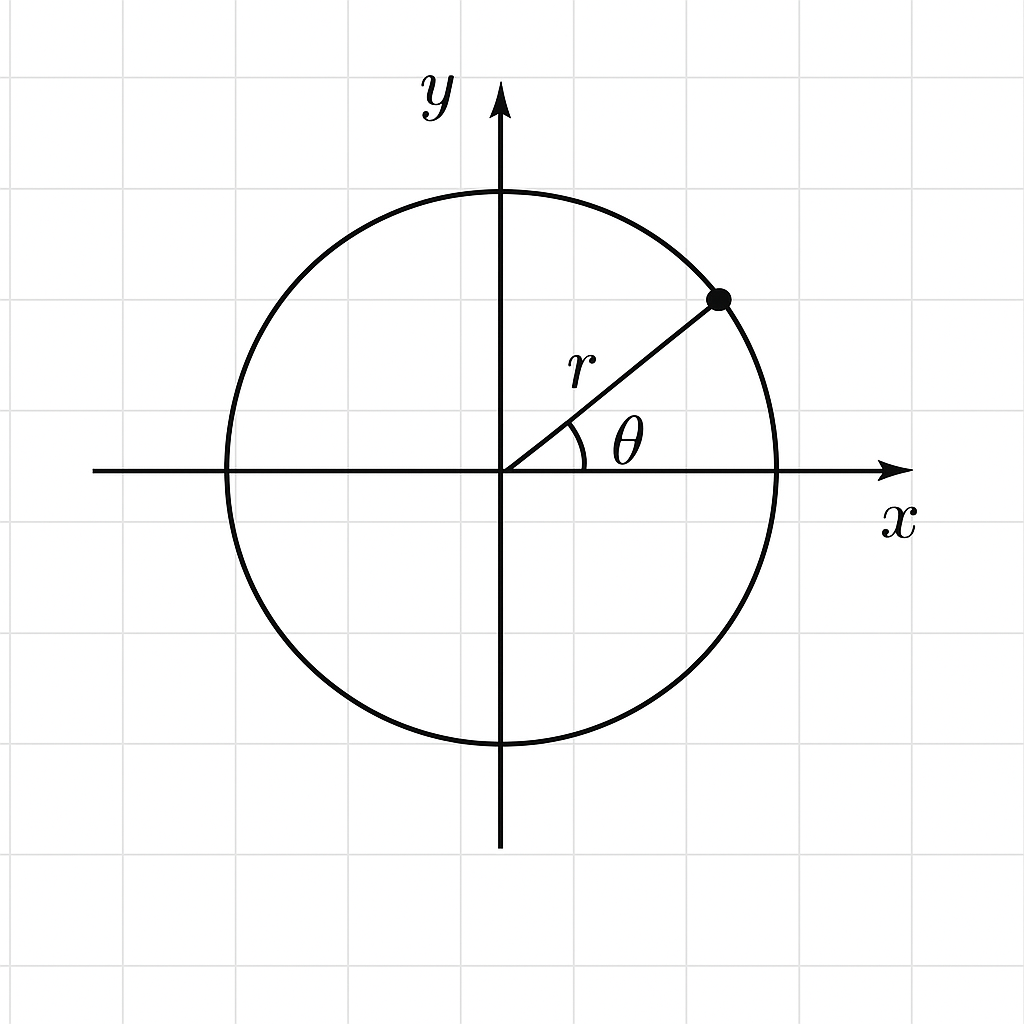
\includegraphics[width=0.4\textwidth]{images/Ch2_polar_coords.png}
\end{center}
It’s clear that \(f\) is a bijection, and \(f\) is continuous. Moreover, the inverse \(g := {f}^{-1}\) is defined as
\[
g\left({a,b}\right)  = \left({\frac{a}{\sqrt{{a}^{2} + {b}^{2}}},\frac{b}{\sqrt{{a}^{2} + {b}^{2}}},\sqrt{{a}^{2} + {b}^{2}}}\right)
\]
which is continuous as well. Therefore, the \(f : {\mathcal{S}}^{1} \times  \left({0,\infty}\right)  \rightarrow  {\mathbb{R}}^{2} \smallsetminus  \{ \mathbf{0}\}\) is a homeomorphism.
\end{example}

\begin{proposition} a ring torus is homeomorphic to the Cartesian product of two circles, say \({S}^{1} \times  {S}^{1} \cong  T\).
\end{proposition}
\begin{figure}[h]
  \centering
  \animategraphics[autoplay,loop,width=0.6\textwidth]{12}{images/torus_frames/frame_}{001}{047}%
  % Fallback static frame (shows in Overleaf preview):
  % 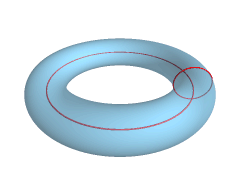
\includegraphics[width=0.6\textwidth]{images/torus_frames/frame_001.png}
  \caption{Ring torus degenerating into a spindle torus.(The animation only works in Adobe.)}
\end{figure}

\begin{proof} 
Let $S^1 \times S^1 = \{(\cos(\theta),\sin(\theta),\cos(\phi),\sin(\phi))\ |\ 0 \leq \theta,\phi <2\pi\}$. The product topology of $S^1 \times S^1$ is just the subspace topology of $\mathbb{R}^4$. Define a mapping \(f : S^1  \times  S^1   \rightarrow  T\) by
\[
f\left({\theta,\phi}\right)  = \left({\left({R + r\cos \theta}\right) \cos \phi,\;\left({R + r\cos \theta}\right) \sin \phi,\;r\sin \theta}\right)
\]
for $R > r$. Denote \(i : T \rightarrow  {\mathbb{R}}^{3}\) as the usual inclusion, then we imply
\[
i \circ  f : \left\lbrack  {0,{2\pi}}\right)   \times  \left\lbrack  {0,{2\pi}}\right)   \rightarrow  {\mathbb{R}}^{3}\text{ is continuous}
\]
Therefore, by \autoref{prop:subspace_equivalent} we imply \(f : \left\lbrack  {0,{2\pi}}\right)   \times  \left\lbrack  {0,{2\pi}}\right)   \rightarrow  T\) is continuous. We can also show it is bijective, and \({f}^{-1}\) is continuous as in the previous example which are left as exercises.
\end{proof}

\begin{proposition} Let \(X \times  Y\) be endowed with product topology. Then the projection mappings defined as
\[
p_X : X \times  Y \rightarrow  X\text{, with }p_X\left({x,y}\right)  = x, \quad \quad 
p_Y : X \times  Y \rightarrow  Y\text{, with }p_Y\left({x,y}\right)  = y
\]
are continuous. Moreover:
\begin{enumerate}
    \item The product topology is the coarsest topology on \(X \times  Y\) such that \(p_X\) and \(p_Y\) are both continuous.

    \item Let \(Z\) be a topological space, then the product topology is the unique topology that the red and the blue line in the diagram commutes:
\begin{center}
\begin{tikzcd}[column sep=large, row sep=large]
& Z \ar[ld, "\color{blue}p_X \circ F"'] \ar[rd, "\color{blue}p_Y \circ F"] \ar[d, "\color{red}F" description] & \\
X & X \times Y \ar[l, "p_X"'] \ar[r, "p_Y"] & Y
\end{tikzcd}
\end{center}
namely, the mapping \(F : Z \rightarrow  X \times  Y\) is continuous iff both \(p_X \circ  F : Z \rightarrow  X\) and
\(p_Y \circ  F : Z \rightarrow  Y\) are continuous.
\end{enumerate}
\end{proposition}

\begin{proof} The first statement of the proposition is easy - for any open \(U\), we imply \(p_X^{-1}\left(U\right)  = U \times  Y \in  {\mathcal{B}}_{X \times  Y} \subseteq  {\mathcal{T}}_{X \times  Y}\), i.e., \(p_X^{-1}\left(U\right)\) is open. The same goes for \(p_Y\).

\begin{enumerate}
    \item  It suffices to show any topology \(\mathcal{T}\) that meets the condition in (2) must contain \({\mathcal{T}}_{\text{product}}\). We imply that For all \(U \in  {\mathcal{T}}_X,V \in  {\mathcal{T}}_Y\),
\[
\left\{  {\begin{array}{l} p_X^{-1}\left(U\right)  = U \times  Y \in  \mathcal{T} \\  p_Y^{-1}\left(V\right)  = X \times  V \in  \mathcal{T} \end{array} \Rightarrow  \left({U \times  Y}\right)  \cap  \left({X \times  V}\right)  = \left({U \cap  X}\right)  \times  \left({Y \cap  V}\right)  = U \times  V \in  \mathcal{T},}\right.
\]
which implies \({\mathcal{B}}_{X \times  Y} \subseteq  \mathcal{T}\). Since \(\mathcal{T}\) is closed for union operation on subsets, we
imply \({\mathcal{T}}_{\text{product}} \subseteq  \mathcal{T}\).

\item First, we show that \({\mathcal{T}}_{\text{product}}\) satisfies the commutative diagram.
\begin{itemize}
\item For the forward direction, by the first statement of the proposition, we imply both \(p_X \circ  F\) and \(p_Y \circ  F\) are continuous, since the composition of continuous functions are continuous as well.

\item For the reverse direction, For all \(U \in  {\mathcal{T}}_X,V \in  {\mathcal{T}}_Y\),
\[
{F}^{-1}\left({U \times  V}\right)  = {\left(p_X \circ  F\right)}^{-1}\left(U\right)  \cap  {\left(p_Y \circ  F\right)}^{-1}\left(V\right),
\]
which is open due to the continuity of \(p_X \circ  F\) and \(p_Y \circ  F\).
\end{itemize}

Next, we show the uniqueness of \({\mathcal{T}}_{\text{product}}\). Let \(\mathcal{T}\) be another topology \(X \times  Y\) satisfying the commutative diagram:
\begin{itemize}
\item Take \(Z = \left({X \times  Y,\mathcal{T}}\right)\), and consider the identity mapping \(F = \mathrm{{id}} : Z \rightarrow  Z\), which is continuous. Therefore \(p_X \circ  \mathrm{{id}}\) and \(p_Y \circ  \mathrm{{id}}\) are continuous, i.e., \(p_X\) and \(p_Y\) are continuous. By (1), we imply \({\mathcal{T}}_{\text{product}} \subseteq  \mathcal{T}\).

\item Take \(Z = \left({X \times  Y,{\mathcal{T}}_{\text{product}}}\right)\), and consider the identity mapping \(F = \mathrm{{id}}\) : \(Z \rightarrow  Z\). Note that \(p_X \circ  F = p_X\) and \(p_Y \circ  F = p_Y\), which is continuous. Therefore, the identity mapping \(F : \left({X \times  Y,{\mathcal{T}}_{\text{product}}}\right)  \rightarrow  \left({X \times  Y,\mathcal{T}}\right)\) is continuous, which implies
\[U = {\operatorname{id}}^{-1}\left(U\right)  \subseteq  {\mathcal{T}}_{\text{product}}\ \text{for all }\ U \in  \mathcal{T}\text{,}
\]
i.e., \(\mathcal{T} \subseteq  {\mathcal{T}}_{\text{product}}\).
\end{itemize}
\end{enumerate}
Consequently, the proof is complete. 
\end{proof}


\begin{definition}[Disjoint Union] Let \(X \times  Y\) be two topological spaces, then the \emph{disjoint union} of \(X\) and \(Y\) is
\[
X\coprod Y := \left({X\times \{ 0\}}\right)  \cup  \left({Y\times \{ 1\}}\right),
\]
where \(\mathcal{T}_{X\coprod Y}\) consists of all \(U \subseteq X \coprod  Y\) satisfying:
\begin{itemize}
    \item \(U \cap  \left({X\times \{ 0\}}\right)\) is open in \(X \times  \{ 0\}\) ; and
    \item \(U \cap  \left({Y\times \{ 1\}}\right)\) is open in \(Y \times  \{ 1\}\).
\end{itemize}
(Exercise: show $\mathcal{T}_{X\coprod Y}$ defines a topology)
\end{definition}
In other words, \(S\) is open in \(X \coprod  Y\) iff \(S\) can be expressed as
\[
S = \left({U\times \{ 0\}}\right)  \cup  \left({V\times \{ 1\}}\right)
\]
where \(U \subseteq  X\) is open and \(V \subseteq  Y\) is open.